\documentclass[a4paper, 12pt]{report}

%%%%%%%%%%%%
% Packages %
%%%%%%%%%%%%

\usepackage[english]{babel}
\usepackage[noheader]{packages/sleek}
\usepackage{packages/sleek-title}
\usepackage{packages/sleek-theorems}
\usepackage{packages/sleek-listings}
\usepackage{kotex}
\usepackage{lipsum}
\usepackage[utf8]{inputenc}
\usepackage[english]{babel}

%%%%%%%%%%%%%%
% Title-page %
%%%%%%%%%%%%%%

\logo{./resources/pdf/logo.pdf}
\institute{Seoul National University}
\faculty{Department of Aerospace Engineering}
\department{Flight Dynamics and Control Laboratory}
\title{Flight Control System Design for Morphing Aircraft}
\subtitle{Development of an SMPC Flap Module for Morphing Wings}
\author{\textit{Author}\\Jihoon \textsc{Lee}\\Seungyun \textsc{Jung}\\Seong-hun \textsc{Kim}\\Hanna \textsc{Lee}}
\supervisor{Yondan Kim}
\context{\small{with\\Ministry of Trade, Industry and Energy\\Korea Evaluation Institute of Industrial Technology\\Korea Aerospace University\\Chungnam National University\\Sejong University\\DBRAIN}\\~\\}
\date{December 31, 2020}

%%%%%%%%%%%%%%%%
% Bibliography %
%%%%%%%%%%%%%%%%

\addbibresource{./resources/bib/references.bib}

%%%%%%%%%%
% Others %
%%%%%%%%%%

\lstdefinestyle{latex}{
	language=TeX,
	style=default,
	%%%%%
	commentstyle=\ForestGreen,
	keywordstyle=\TrueBlue,
	stringstyle=\VeronicaPurple,
	emphstyle=\TrueBlue,
	%%%%%
	emph={LaTeX, usepackage, textit, textbf, textsc}
}

\FrameTBStyle{latex}

\def\tbs{\textbackslash}

%%%%%%%%%%%%
% Document %
%%%%%%%%%%%%

\begin{document}
	\maketitle
	\romantableofcontents
	
	\chapter{Introduction}
	일반적으로 고정익 항공기를 위한 제어시스템을 설계하는 경우 사전에 정의된 운용점 근방에서 수학적 모델을 구축하고, 이를 기반으로 주어진 임무에 따라 요구되는 비행성능을 만족하도록 제어기를 설계한다.
	그러나 모핑 항공기의 경우 변형 가능한 모든 형상에 대해 개별적으로 공력 모델을 얻고 제어기를 설계하는 데에 시간과 비용이 지나치게 많이 소요된다.
	특히 항공기가 모핑을 하는 과정에서 나타나는 다양한 시변 효과는 동역학 모델을 시불변 시스템으로 가정하는 데서 출발하는 많은 기법들의 직접적인 적용을 어렵게 한다~\cite{seigler_analysis_2009,chakravarthy_time-varying_2012}.
	지난 수년간 이러한 어려움을 가진 모핑 항공기 제어시스템 설계를 위해  선형시변시스템에 기반하여 제어기를 설계하거나~\cite{jiang_systematic_2015,lee_linear_2019}, 파라미터화 된 모핑 변수를 동역학 모델에 포함시키거나 외란으로 간주하여 비선형 제어기를 설계하는 방식~\cite{wu_modified_2017,lee_neural_2019,jung_disturbance_2020} 등이 제안되었다.
	
	\begin{figure}[h]
		\centering
		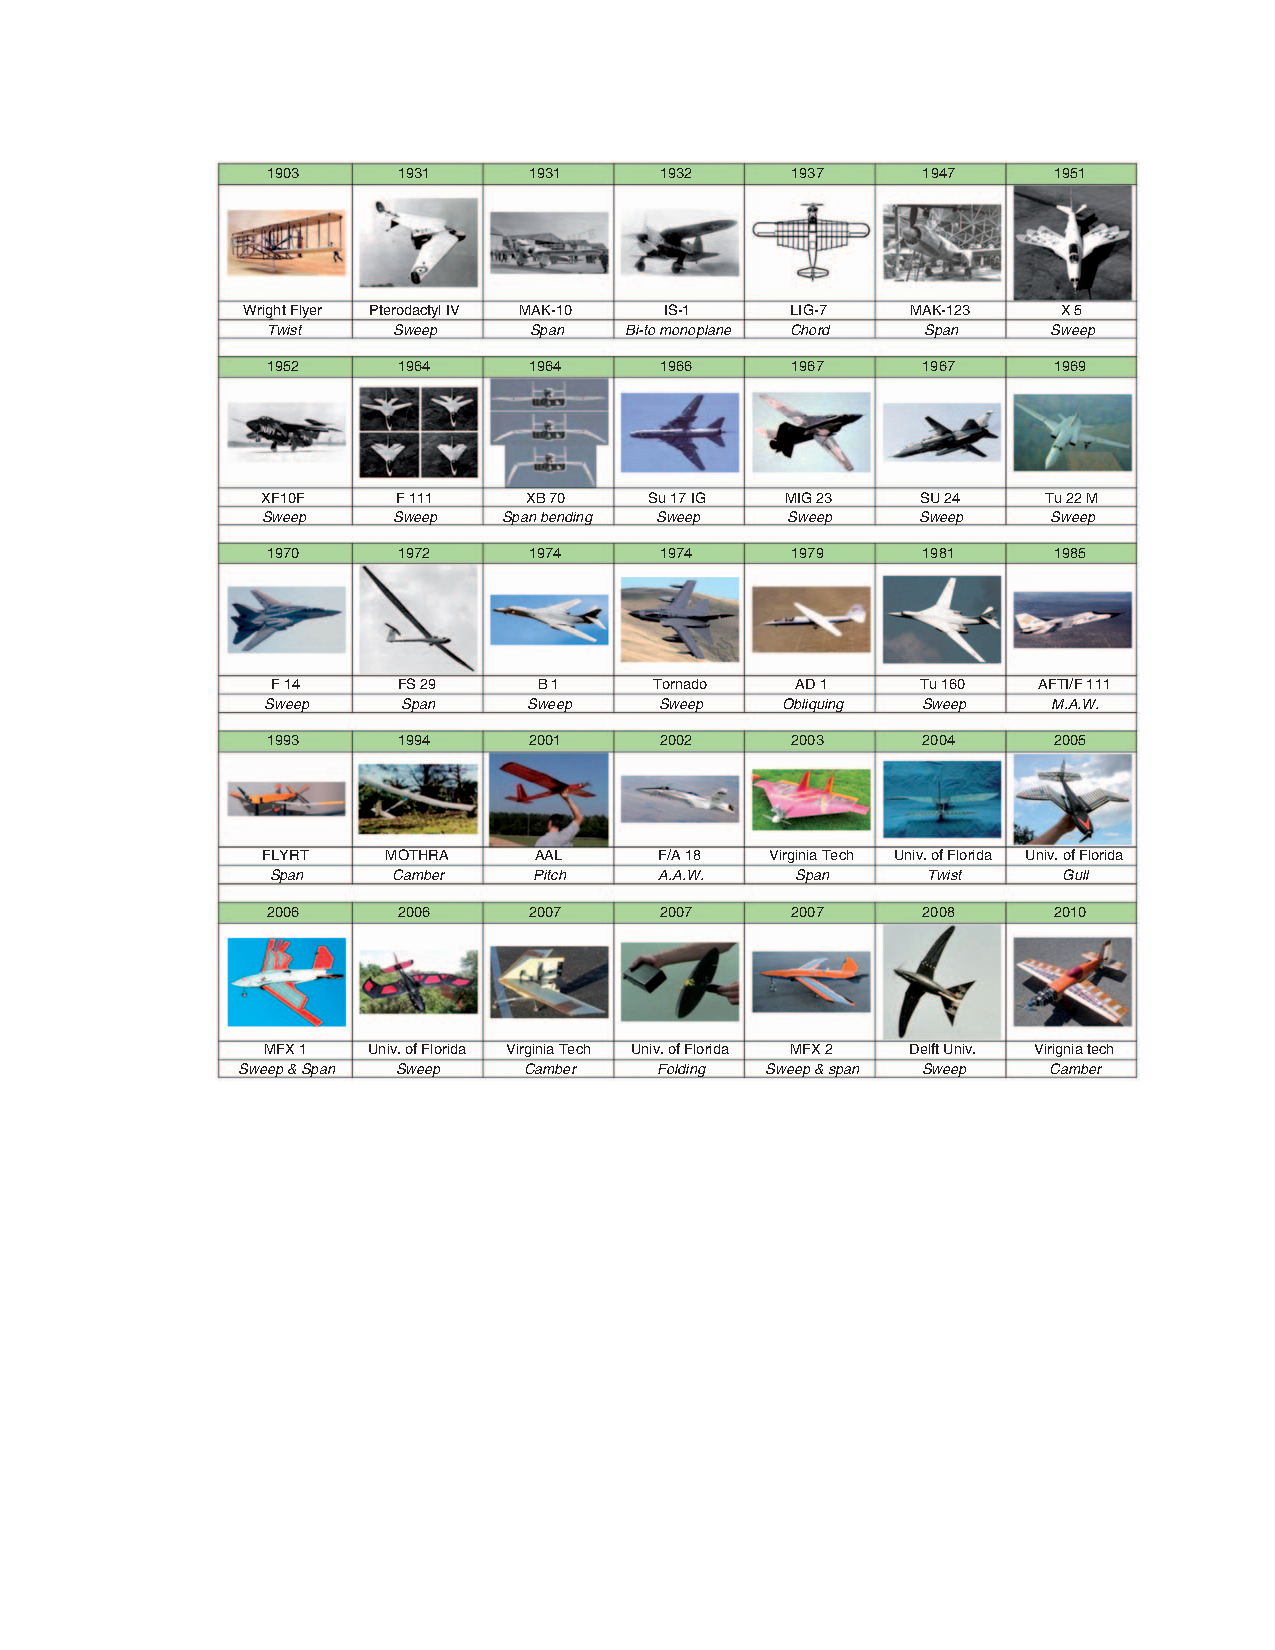
\includegraphics[width=0.6\textwidth]{./resources/pdf/history.pdf}
		\caption{Timeline of fixed wing aircraft implementing morphing technologies \cite{barbarino2011review}}.
		\label{fig:history}
	\end{figure}
	
	본 문서에서는 모핑 항공기를 위한 선형 및 비선형 비행제어 시스템 설계 방법에 대해 기술한다.
	제어 시스템의 설계는 지난 수십년간 높은 안정성과 제어 성능을 보여준 수학적 모델 기반 설계 기법을 도입한다.
	이를 위해선 실제 모핑 항공기의 동적 거동을 최대한 정확히 모사하는 동역학 모델이 필요하다.
	모핑 항공기의 동역학 특성을 물리적으로 잘 고려한 T. M. Siegler와 D. A. Neal의 모델링 기법~\cite{seigler_modeling_2007-1}을 참고하여, 스팬이나 스윕 모핑에 따라 변화하는 공력 중심과 관성 모멘트, 공력을 고려한 선형, 비선형 모핑 항공기 모델을 도출한다.
	이후 각 절에서는 도출된 선형 및 비선형 모델에 기반하여 선형 최적제어기와 비선형 동적모델 역변환 제어기를 설계한다.
	선형 최적제어기는 직관적인 성능 지표를 통해 모핑 상황에서 항공기가 우선적으로 제어해 주어야 할 상태변수를 선정할 수 있으며, 제어기 자체가 매우 강건하기 때문에 정확한 모델링이 힘든 모핑 항공기 제어 시스템으로 적절하다.
	비선형 동적 모델 역변환 제어기는 선형 최적제어기에 비해 모델 정확도에 대한 의존도가 높지만, 비선형 모델을 직접적으로 사용함으로써 모핑 항공기의 넓은 비행영역 전반에 걸쳐 유효한 성능을 가지도록 할 수 있다.
	마지막으로 모핑 항공기 제어 시스템 설계에 위 기법들을 사용함에 있어 주의할 점들에 대해 서술하였다.
	
	\chapter{Modeling}
	
	모핑 항공기를 위한 비행제어시스템을 개발하기 위해서는 수학적 모델링이 선행되어야 한다. 
	기본적으로 수학적 모델은 물리법칙에 의거하여 만들어지고 실험 데이터를 이용하여 개선된다. 
	수학적 모델은 분명한 한계를 가지고있으며, 제어시스템 개발 과정에서 이러한 한계점을을 적절히 고려하는 것이 중요하다.
	개발된 모델은 제어시스템 설계에 사용될 뿐만 아니라 초기 설계 단계에 있는 항공기의 성능을 평가하고 더 나아가 항공기 설계를 개선하는데도 사용된다.
	본 장에서는 일반 항공기와 다른 모핑 항공기의 수학적 모델을 도출하는 과정을 다룬다.
	먼저 실험 데이터를 이용하여 모핑 항공기에 작용하는 힘과 모멘트를 모델링하고, 이를 사용하여 비선형 모델을 유도한 이후, 선형화 과정을 거쳐 선형 모델을 도출한다.
	
	\section{Force and Moment}
	
	모핑 항공기에 작용하는 공기역학적 힘과 모멘트는 모핑 항공기의 자세 및 형상에 영향을 받는다.
	공력은 동체와 동체 주변 공기 흐름의 상대운동에 의해 발생하므로 동체 좌표계보다는 바람 좌표계에서 다음과 같이 표현하는 것이 일반적이다.
	\begin{align}
		D =& \bar{q}SC_D \\
		C =& \bar{q}SC_C \\
		L =& \bar{q}SC_L \\
		l_w =& \bar{q}SbC_l \\
		m_w =& \bar{q}S\bar{c}C_m \\
		n_w =& \bar{q}SbC_n
	\end{align}
	여기서 $D$, $C$, $L$은 각각 항력, 측력, 양력을, $l$, $m$, $n$은 롤축, 피치축, 요축 모멘트를, $q$는 동압을, $S$, $b$, $\bar{c}$는 각각 주익의 면적, 스팬 길이, 코드 길이를 나타낸다.
	위 식의 무차원 공기역학 계수들은 일반적으로 해석적 기법, 전산유체역학, 풍동시험, 비행시험 등을 통해 얻어지는데, 완전한 모델링을 위해서는 이러한 기법들을 다양한 비행조건(고도, 마하수 등)과 받음각 및 옆미끄럼각을 가지는 경우에 대해 폭넓게 적용해야 한다.
	이때 모핑 항공기의 경우 형상 변화에 따른 공력계수의 변화도 반영이 되어야하므로 일반 항공기의 경우보다 시험에 소요되는 시간과 비용이 증가하게 된다.
	본 문서에서는 적절한 공력계수 모델이 이미 주어졌다고 가정하고 수학적 모델을 도출한다.
	
	\section{Nonlinear Model}
	
	모핑 항공기의 동체 좌표계에서의 상태변수 벡터는 다음과 같이 나타낼 수 있다.
	\begin{equation}
		X = [U \quad V \quad W \quad \phi \quad \theta \quad \psi \quad P \quad Q \quad R \quad p_N \quad p_E \quad p_D]
	\end{equation}
	6자유도 운동방정식은 동체 좌표계에서 다음과 같이 나타낼 수 있다 \cite{stevens2015aircraft}.
	\begin{align}
		\dot{U} =& RV-QW-g_D\sin\theta+(X_A+X_T)/\text{m} \\
		\dot{V} =& -RU+PW-g_D\sin\phi+(Y_A+Y_T)/\text{m} \\
		\dot{W} =& QU-PV+g_D\cos\phi\cos\theta+(Z_A+Z_T)/\text{m} \\
		\dot{\phi} =& P+\tan\theta(Q\sin\phi+R\cos\phi) \\
		\dot{\theta} =& Q\cos\phi-R\sin\phi \\
		\dot{\psi} =& (Q\sin\phi+R\cos\phi)/\cos\theta \\
		\Gamma\dot{P} =& J_{xz}[J_x-J_y+J_z]PQ-[J_z(J_z-J_y)+J_{xz}^2]QR+J_zl+J_{xz}n \\
		J_y\dot{Q} =& (J_z-J_x)PR-J_{xz}(P^2-R^2)+m \\
		\Gamma\dot{R} =& [(J_x-J_y)J_X+J_{xz}^2]PQ-J_{xz}[J_x-J_y+J_z]QR+J_{xz}l+J_xn \\ 
		& \cdot \Gamma = J_xJ_z-J_{xz}^2 \nonumber \\ 
		\dot{p}_N =& Uc\theta c\psi+V(-c\phi s\psi+s\phi s\theta c\psi)+W(s\phi s\psi+c\phi s\theta c\psi) \\
		\dot{p}_E =& Uc\theta s\psi+V(c\phi c\psi+s\phi s\theta s\psi)+W(-s\phi c\psi+c\phi s\theta s\psi) \\
		\dot{p}_D =& -Us\theta+Vs\phi c\theta+Wc\phi c\theta
	\end{align}
	여기서 $U$, $V$, $W$는 속도의 동체 좌표계 성분, $\phi$, $\theta$, $\psi$는 자세의 3-2-1 오일러 각, $P$, $Q$, $R$은 각속도의 동체 좌표계 성분, $p_N$, $p_E$, $p_D$는 위치의 NED 좌표계 성분, $X_A$, $Y_A$, $Z_A$는 공력의 동체 좌표계 성분, $X_T$, $Y_T$, $Z_T$는 추력의 동체 좌표계 성분, $\text{m}$은 질량, $g_D$는 중력가속도의 local down 방향 성분, $J_x$, $J_y$, $J_z$, $J_{xz}$는 동체 좌표계에 대해 정의된 inertia matrix의 성분이다. 이때, 비대칭 모핑으로 인해 좌우 대칭이 깨질 경우 $J_xy$ 성분의 크기가 무시할 수 없을 정도로 커질 수 있다.
	
	\section{Linear Model}
	
	정상 수평비행 상태에 대해 수치적 선형화를 수행하면 종방향과 횡방향 운동을 분리해서 다룰 수 있다.
	종방향 상태변수 벡터와 제어입력 벡터는 다음과 같이 정의된다.
	\begin{align}
		x_{lon} =& \begin{bmatrix}
			\alpha && q && V_T && \theta
		\end{bmatrix} \\
		u_{lon} =& \begin{bmatrix}
			\delta_e && \delta_t
		\end{bmatrix}
	\end{align}
	종방향 운동은 다음과 같은 선형 방정식으로 나타낼 수 있다.
	\begin{equation}
		x=A_{lon} x_{lon}+B_{lon} u_{lon}
	\end{equation}
	이때 종방향 계수 행렬들은 수치적으로 얻어진다.
	횡방향 상태변수 벡터와 제어입력 벡터는 다음과 같이 정의된다.
	\begin{align}
		x_{lat} =& \begin{bmatrix}
			\beta && \phi && p && r
		\end{bmatrix} \\
		u_{lat} =& \begin{bmatrix}
			\delta_a && \delta_r
		\end{bmatrix}
	\end{align}
	횡방향 운동은 다음과 같은 선형 방정식으로 나타낼 수 있다.
	\begin{equation}
		x=A_{lat} x_{lat}+B_{lat} u_{lat}
	\end{equation}
	이때 횡방향 계수 행렬들은 수치적으로 얻어진다.	
	
	\chapter{Linear Quadratic Regulator}
	
	항공기의 수학적 모델링이 선행되면 도출한 수학적 모델을 기반으로 비행제어시스템을 설계할 수 있다.
	선형 시스템의 경우, 종방향과 횡방향으로 분리된 선형 모델을 통해 주어진 선형 모델 근방에서의 종방향 제어시스템과 횡방향 제어시스템을 나누어 설계한다.
	설계한 제어기는 미리 주어진 궤적을 추종하는 제어입력을 도출하는 것을 목표로 한다.
	
	\begin{figure}[h]
		\centering
		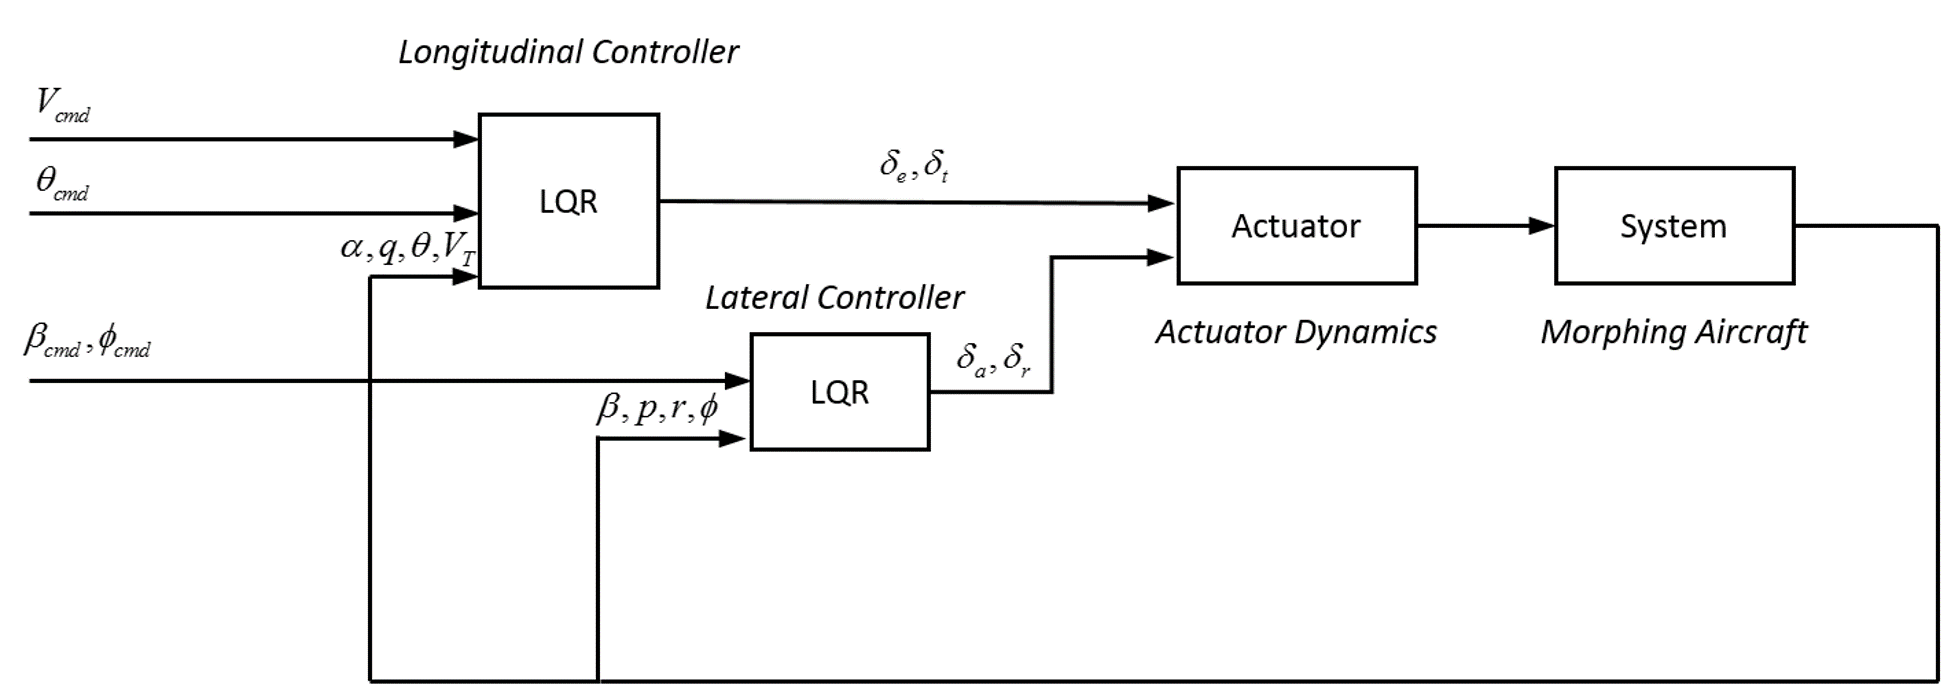
\includegraphics[width=0.8\textwidth]{./resources/pdf/lqr.png}
		\caption{Block diagram of LQR for morphing aircraft.}
		\label{fig:lqr}
	\end{figure}
	
	\section{Derivation of Optimal Control}
	
	비행제어기 설계시 항공기의 선형 모델이 주어졌을 때, 대표적으로 선형 최적 제어기(linear quadratic regulator, LQR)를 고려할 수 있다.
	선형 최적 제어기는 고려한 성능지수에 대해 이를 최소화하도록 제어기를 설계하는 기법이다. 
	종방향과 횡방향 시스템의 상태공간 모델을 구성하는 값들은 다르지만 시스템의 모델에 따른 설계 방식은 모두 동일하다. 
	다음과 같은 선형 모델을 고려하자.
	\begin{equation}
		\dot{x}=Ax+Bu
	\end{equation}
	최적 제어기 설계를 위해 다음과 같은 quadratic form의 성능지수를 고려한다.
	\begin{equation}
		J=\frac{1}{2}\int_0^{\infty}(x^TQx+u^TRu)dt
	\end{equation}
	여기서 $Q$와 $R$은 각각 상태변수와 제어입력에 대한 가중행렬을 나타내며, $Q\geq0,\ R>0$을 만족한다. 
	가중행렬의 성분을 적절히 설계하여 최적 제어기의 성능을 개선시킬 수 있다.
	즉, LQR 문제는 다음과 같은 최적 제어 문제로 표현할 수 있다.
	\begin{equation}
		\begin{aligned}
			&\mathrm{minimize} \hspace{1em} J\\
			&\mathrm{s.t} \hspace{1em} \dot{x}=Ax(t)+Bu(t),\ x(0)=x_0
		\end{aligned}
	\end{equation}
	정상상태를 고려하면, 최적 제어 문제는 다음과 같은 algebraic Ricatti equation으로 표현할 수 있다.
	\begin{equation}
		PA+A^TP-PBR^{-1}B^TP+Q=0
	\end{equation}
	위의 식은 다음과 같은 Lyapunov 방정식을 푸는 것과 같다.
	\begin{equation}
		PS+S^TP=-Q-K^TRK
	\end{equation}
	여기서 $S=A-BK$이고, 방정식을 풀어 $P$와 제어이득 $K$를 차례로 계산할 수 있다.
	결과적으로 따라서 다음과 같은 형태의 최적 제어입력을 도출할 수 있다.
	\begin{equation}
		u(t)=-Kx(t)=-R^{-1}B^TPx(t)
	\end{equation}
	
	\section{Application to Morphing Aircraft}
	
	LQR 기법의 성능을 검증하기위해 가변스팬 모핑 항공기의 자세제어 시뮬레이션을 수행하였다.
	먼저 최소스팬 모델에 대해 설계된 제어기를 이용해 최소스팬 상태의 모핑 항공기의 피치업 기동을 수행하였으며, Fig. \ref{fig:pitching}에서와 같이 피치각 10도 계단 명령을 잘 추종하는것을 볼수 있다.
	다음으로 최소스팬 모델에 대해 설계된 제어기를 이용해 최대스팬 상태의 모핑 항공기의 롤링 기동을 수행하였으며, Fig. \ref{fig:rolling}에서와 같이 롤각 20도 계단 명령을 잘 추종하는것을 볼수 있다.
	
	\begin{figure}[h]
		\centering
		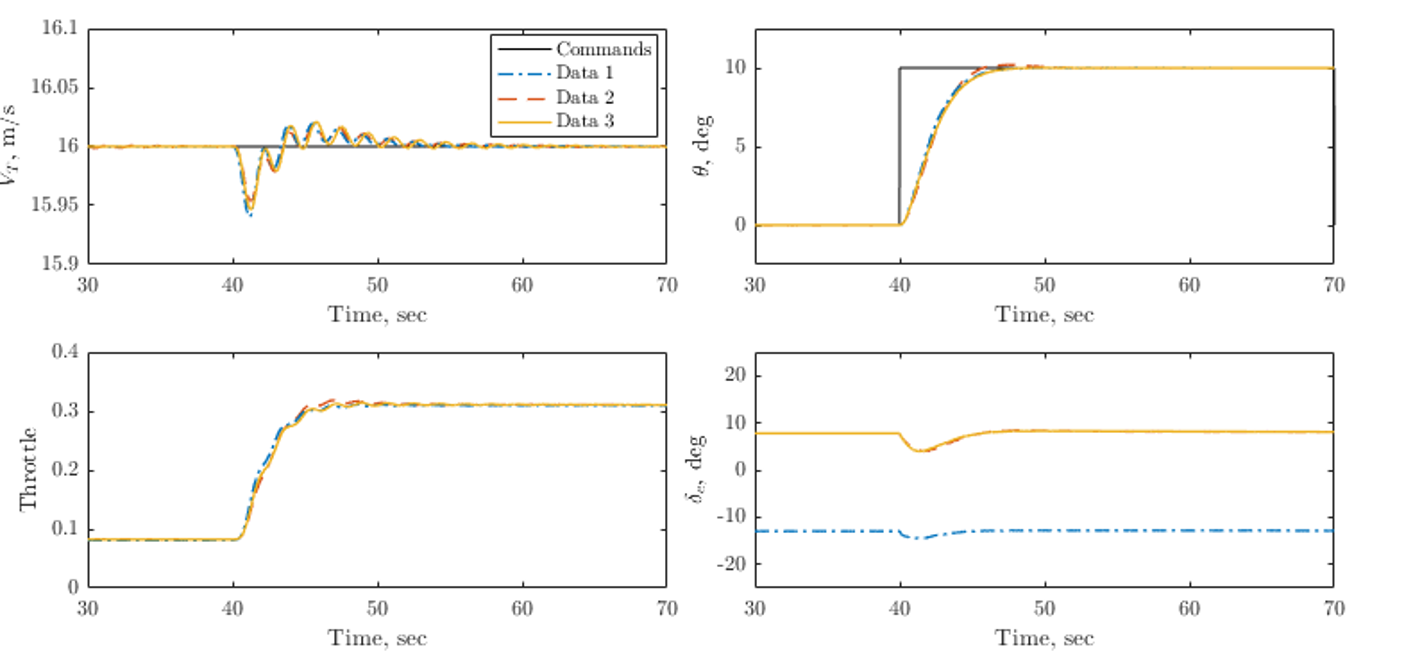
\includegraphics[width=0.55\textwidth]{./resources/pdf/pitching.png}
		\caption{Pitching maneuver.}
		\label{fig:pitching}
		\centering
		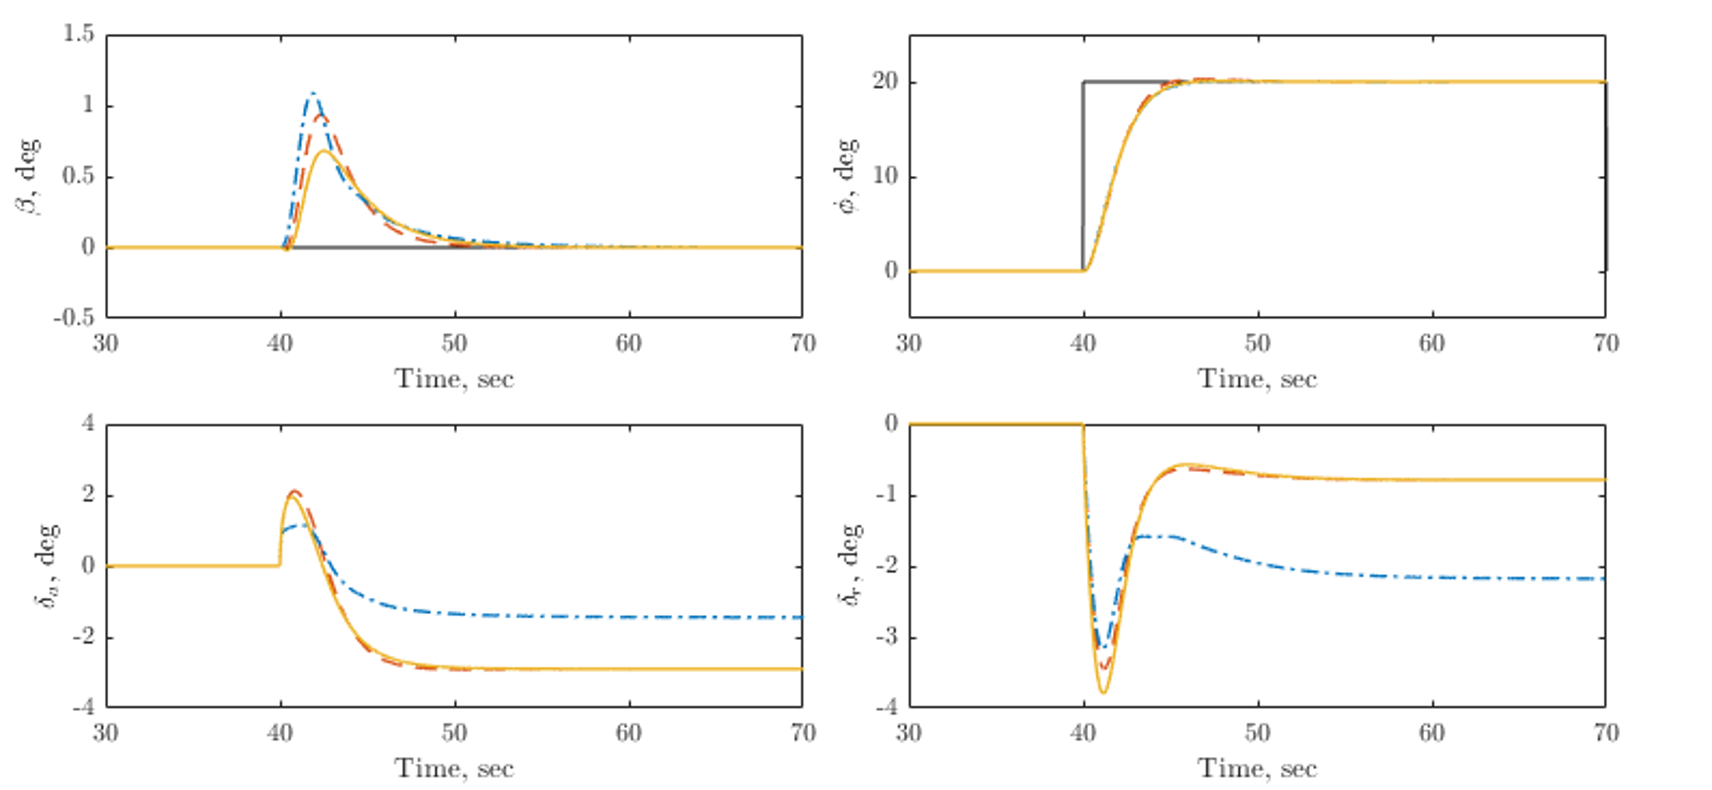
\includegraphics[width=0.55\textwidth]{./resources/pdf/rolling.png}
		\caption{Rolling maneuver.}
		\label{fig:rolling}
	\end{figure}
	
	선형 최적 제어기는 주어진 모델을 이용해 안정성을 보장하는 최적의 제어이득을 쉽게 구할 수 있다는 장점이 있으며, 높은 강건성이 보장되기 때문에 다양한 분야에 폭넓게 적용되어왔다.
	그러나, 이러한 모델기반 제어 기법의 경우 모델에 대한 정확한 정보를 아는 것이 필수적이며, 비선형성이 큰 모델에 대해서는 제어 성능을 보장하기 어렵다.
	
	\chapter{Nonlinear Dynamic Inversion}
	
	비행제어기 설계시 고려되는 대표적인 비선형 제어방법으로는 비선형 동적 모델역변환 제어(nonlinear dynamic inversion, NDI)기법이 있다. 비선형 동적 모델역변환 제어 기법은 적절한 비선형좌표변환을 이용하여 주어진 비행동역학을 새로운 좌표계에서 표현한 후 제어입력을 설계하는 제어 방식으로, 설계되는 제어 입력은 비선형 비행동역학을 상쇄하는 항과 시스템을 안정화 시키는 새로운 제어항으로 구성된다. 비선형 동적 모델역변환 제어를 이용할 경우 상태공간 전체에서 유효한 성능을 보이는 비행 제어기를 설계할 수 있다는 점이 장점이다. 그러나 비선형 동적 모델역변환 제어기법이 잘 동작하기 위해서는 높은 정확도의 비행동역학 모델 정보가 요구되며 비행동역학 모델의 정확도가 낮으면 비선형 동적 모델역변환 제어기법의 성능이 저하되고 경우에 따라서는 제어기의 안전성마저도 보장되지 않을 수 있다는 것이 비선형 동적 모델역변환 제어기법의 잘 알려진 단점이다.
	
	\section{General Theory of NDI}
	
	일반적으로 비선형 동적 모델역변환 기법을 적용하기 위한 다음과 같은 비선형 시불변 입력-아핀(input-affine) 시스템을 고려하자.
	\begin{equation}\label{Eq:NDI_sys}
		\begin{split}
			\dot{\mathbf{x}} &= f(\mathbf{x}) + G(\mathbf{x})\mathbf{u} \\
			\mathbf{y} &= h(\mathbf{x})
		\end{split}
	\end{equation}
	\begin{equation}\label{Eq:InputMTRX}
		G(\mathbf{x}) =
		\begin{bmatrix}
			g_{1}(\mathbf{x}), & \dots & ,g_{m}(\mathbf{x})
		\end{bmatrix}
	\end{equation}
	\begin{equation}\label{Eq:outputMTRX}
		h(\mathbf{x}) =
		\begin{bmatrix}
			h_{1}(\mathbf{x}), & \dots & ,h_{m}(\mathbf{x})
		\end{bmatrix}^{T}
	\end{equation}
	단, $\mathbf{x} \in \mathbb{R}^{n\times1}$, $\mathbf{u} \in \mathbb{R}^{m\times1}$, $f(\cdot) \in \mathbb{R}^{n\times1}$, $h(\cdot) \in \mathbb{R}^{m\times1}$, $g_{i}(\cdot) \in \mathbb{R}^{n\times1}$, 그리고 $h_{i}(\cdot) \in \mathbb{R}\,\,(i=1,\cdot\cdot\cdot,m)$. 여기서 $\mathbf{y}$는 제어하고자 하는 성능 출력(performance output)이다. 다음과 같은 연산을 고려하자.
	\begin{equation}\label{Eq:output_dere}
		\begin{split}
			\dot{y}_{i} &= L_{f}h_{i} + \sum_{j=1}^{m}( L_{g_{j}}h_{i} )u_{j} = L_{f}h_{i} \\
			\ddot{y}_{i} &= L_{f}^{2}h_{i} + \sum_{j=1}^{m}L_{g_{j}}( L_{f}h_{i} )u_{j} = L_{f}^{2}h_{i} \\
			\vdots  \\
			y_{i}^{(\lambda_{i})} &= L_{f}^{\lambda_{i}}h_{i} + \sum_{j=1}^{m}L_{g_{j}}( L_{f}^{\lambda_{i}-1}h_{i} )u_{j}
		\end{split}
	\end{equation}
	단, 상대차수 $\lambda_{i}$는 각각의 $h_{i}$에 대해서 최소 하나의 $j \in \{1,2,\cdot\cdot\cdot,m\}$에 대해 다음 수식을 만족하는 최소 정수로 정의된다.
	\begin{equation}\label{Eq:rela_deg_cond}
		L_{g_{j}}( L_{f}^{\lambda_{i}-1}h_{i} ) \neq 0
	\end{equation}
	또한, $\boldsymbol{\lambda}=(\lambda_{1},\lambda_{2},\cdot\cdot\cdot,\lambda_{m})$은 벡터 상대차수로 정의된다. 이제, 각각의 성능 출력을 시간에 대해 $\lambda_{i}$번 미분하고 얻어진 출력 동역학은 다음과 같이 쓰여질 수 있다.
	\begin{equation}\label{Eq:output_dyn}
		\begin{split}
			\begin{bmatrix}
				y_{1}^{(\lambda_{1})} \\
				y_{2}^{(\lambda_{2})} \\
				\vdots \\
				y_{m}^{(\lambda_{m})}
			\end{bmatrix}
			&=
			\begin{bmatrix}
				L_{f}^{\lambda_{1}}h_{i} \\
				L_{f}^{\lambda_{2}}h_{i} \\
				\vdots \\
				L_{f}^{\lambda_{m}}h_{i}
			\end{bmatrix}
			+
			\begin{bmatrix}
				L_{g_{1}}( L_{f}^{\lambda_{1}-1}h_{1} ) & \dots & L_{g_{m}}( L_{f}^{\lambda_{1}-1}h_{1} ) \\
				\vdots & \ddots & \vdots \\
				L_{g_{1}}( L_{f}^{\lambda_{m}-1}h_{m} ) & \dots & L_{g_{m}}( L_{f}^{\lambda_{m}-1}h_{m} )
			\end{bmatrix}
			\mathbf{u} \\
			&\triangleq f^{*}(\mathbf{x}) + G^{*}(\mathbf{x})\mathbf{u}
		\end{split}
	\end{equation}
	행렬 $G^{*}(\mathbf{x})$가 nonsingular하다면 다음과 같은 제어입력을 설계할 수 있다.
	\begin{equation}\label{Eq:NDI_input1}
		\mathbf{u} = G^{*}(\mathbf{x})^{-1}\{ -f^{*}(\mathbf{x}) + \boldsymbol{\nu} \}
	\end{equation}
	여기서 $-f^{*}(\mathbf{x})$이 비선형 비행동역학을 상쇄하는 항을 나타내며 $\boldsymbol{\nu}$이 시스템을 안정화 하는 새로운 제어항을 나타낸다. 새로운 제어항 $\boldsymbol{\nu}$는 설계자에 따라 다양한 방식으로 설계되어 질 수 있다. 만약
	\begin{equation}\label{Eq:rela_deg_full}
		\sum_{i=1}^{m}\lambda_{i} = n
	\end{equation}
	이 만족된다면 출력 동역학을 안정화 시키는 제어입력을 설계함으로 전체 시스템을 안정화 시킬 수 있다. 그러나 만약
	\begin{equation}
		\sum_{i=1}^{m}\lambda_{i} < n
	\end{equation}
	이라면 단순히 출력 동역학을 안정화 시키는 제어입력만으로는 전체 시스템을 안정화 시킬 수 없으며 내부 동역학(internal dynamics)이 전체 시스템의 안정성에 영향을 끼치게된다.
	
	\section{Application to Longitudinal Control for Aircraft}
	
	이제 비선형 동적 모델역변환 제어기법을 항공기의 종방향운동 제어에 적용하기위해 다음과 같은 항공기 종방향 운동방정식을 고려하자.
	\begin{equation}
		\dot{V}_{T} = \frac{T\cos{\alpha}-D}{m} - \frac{\mu\sin{\gamma}}{r^{2}}
	\end{equation}
	\begin{equation}
		\dot{\gamma} = \frac{L+T\sin{\alpha}}{mV_{T}} - \frac{(\mu-rV_{T}^{2})\cos{\gamma}}{r^{2}V_{T}}
	\end{equation}
	\begin{equation}
		\dot{h} = V_{T}\sin{\gamma}
	\end{equation}
	\begin{equation}
		\dot{\alpha} = q-\dot{\gamma}
	\end{equation}
	\begin{equation}
		\dot{q} = \frac{M_{yy}}{J_{yy}}
	\end{equation}
	한편, 제어하고자 하는 성능 출력을 $V_{T}$와 $h$로 정의하면, 전체 시스템을 안정화 하기 위한 상대차수 조건(Eq.~\eqref{Eq:rela_deg_full})이 잘 정의되기 위해 다음과 같은 2차 엔진 동역학 모델이 추가적으로 고려될 필요가 있다.
	\begin{equation}
		\delta\ddot{T} = k_{1}\delta\dot{T} + k_{2}\delta T + k_{3}\delta T_{\text{com}}
	\end{equation}
	이러한 모델을 바탕으로 비선형 동적 모델역변환 제어기법을 적용하기 위해 성능 출력 $V_{T}$ 와 $h$를 시간에 대해 각각 미분하면 $V_{T}$ 와 $h$의 상대차수는 각각 3과 4임을 알 수 있으며, 전체 시스템 차수가 7차이므로 Eq.~\eqref{Eq:rela_deg_full}을 만족한다. 따라서 출력 동역학은 다음과 같다.
	\begin{equation}
		\begin{split}
			\begin{bmatrix}
				\dddot{V}_{T} \\
				h^{(4)}
			\end{bmatrix}
			&=
			\begin{bmatrix}
				f_{V_{T}} \\
				f_{h}
			\end{bmatrix}
			+
			\begin{bmatrix}
				b_{11} & b_{12} \\
				b_{21} & b_{22}
			\end{bmatrix}
			\begin{bmatrix}
				\delta T_{\text{com}}\\
				\delta_{e}
			\end{bmatrix}
			\\
			&\triangleq f^{*}(\mathbf{x}) + G^{*}(\mathbf{x})\mathbf{u}
		\end{split}
	\end{equation}
	따라서 비선형 동적 모델역변환 제어입력은 다음과 같이 설계되어 질 수 있다.
	\begin{equation}
		\begin{bmatrix}
			\delta T_{\text{com}}\\
			\delta_{e}
		\end{bmatrix}
		=
		\begin{bmatrix}
			b_{11} & b_{12} \\
			b_{21} & b_{22}
		\end{bmatrix}^{-1}
		\Bigg\{
		\begin{bmatrix}
			-f_{V_{T}} \\
			-f_{h}
		\end{bmatrix}
		+
		\begin{bmatrix}
			\nu_{1} \\
			\nu_{2}
		\end{bmatrix}
		\Bigg\}
	\end{equation}
	보다 구체적인 수식은 \cite{Wang2000}을 참조한다. 더 나아가 종방향운동뿐 아니라 일반적인 항공기의 6자유도 운동방정식에 time scale 분리를 적용한 비선형 동적 모델역변환 제어기법에 대한 내용은 \cite{Snell1992}을 참고한다. \par
	
	NDI 기반 제어시스템의 성능을 검증하기위해 가변스팬 모핑 항공기에 대해 수치 시뮬레이션을 수행하였다.
	먼저 Fig. \ref{fig:highgturn_trj}, \ref{fig:highgturn1}, \ref{fig:highgturn2}에서는 최소스팬 상태에서는 모핑 항공기가 실속에 빠지지만 비행 중에 적절히 형상을 변형하는 경우 실속에 빠지는 것을 막을 수 있음을 확인할 수 있다.
	다음으로 Fig. \ref{fig:pushover_trj}, \ref{fig:pushover}에서 최소 및 최대스팬 상태의 모핑 항공기에 대해 설계된 제어기가 잘 작동함을 확인할 수 있다.
	
	\begin{figure}[!h]
		\centering
		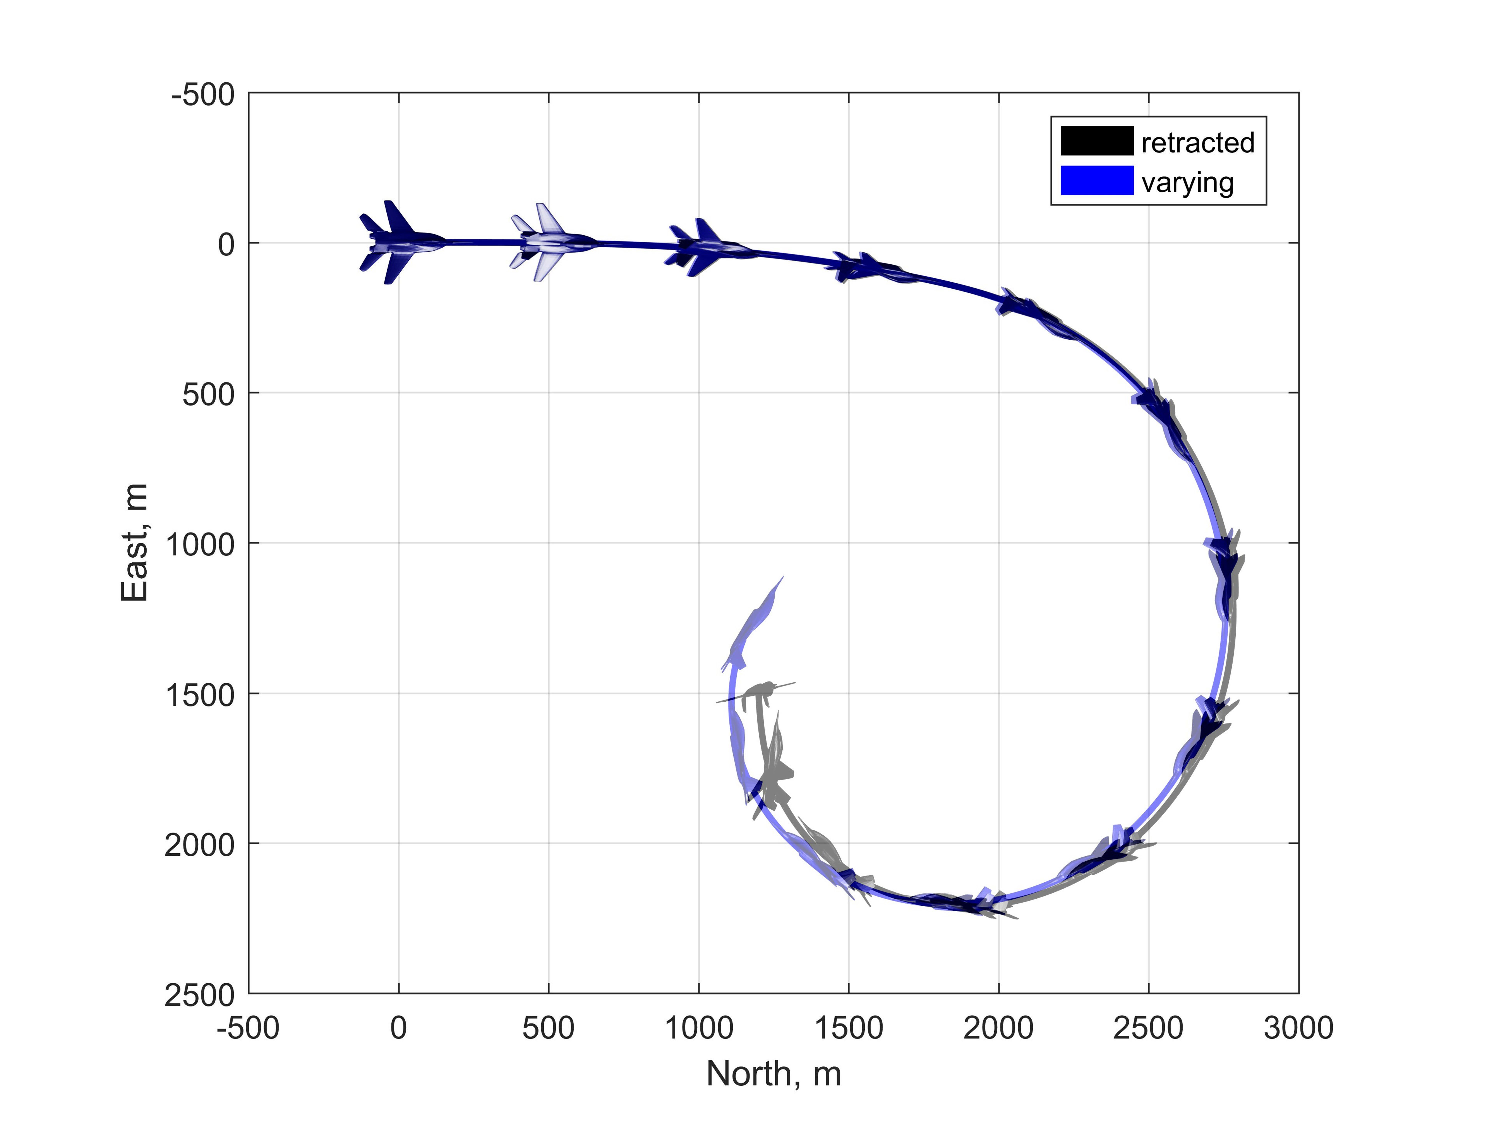
\includegraphics[width=0.6\textwidth]{./resources/pdf/highgturn_trj.pdf}
		\caption{High-g turn maneuver trajectory.}
		\label{fig:highgturn_trj}
		\centering
		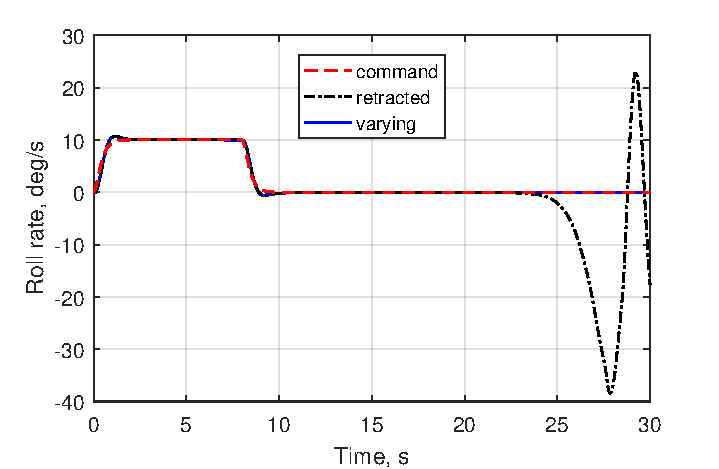
\includegraphics[width=0.6\textwidth]{./resources/pdf/highgturn1.pdf}
		\caption{Roll rate in high-g turn maneuver.}
		\label{fig:highgturn1}
		\centering
		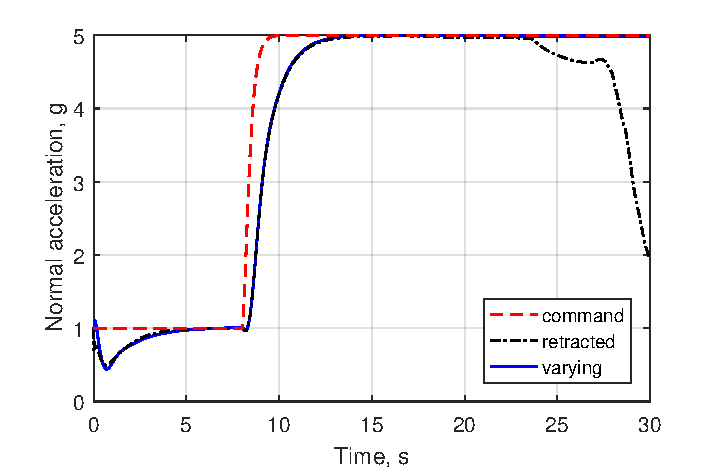
\includegraphics[width=0.6\textwidth]{./resources/pdf/highgturn2.pdf}
		\caption{Normal acceleration in high-g turn maneuver.}
		\label{fig:highgturn2}
	\end{figure}
	\begin{figure}[!t]
		\centering
		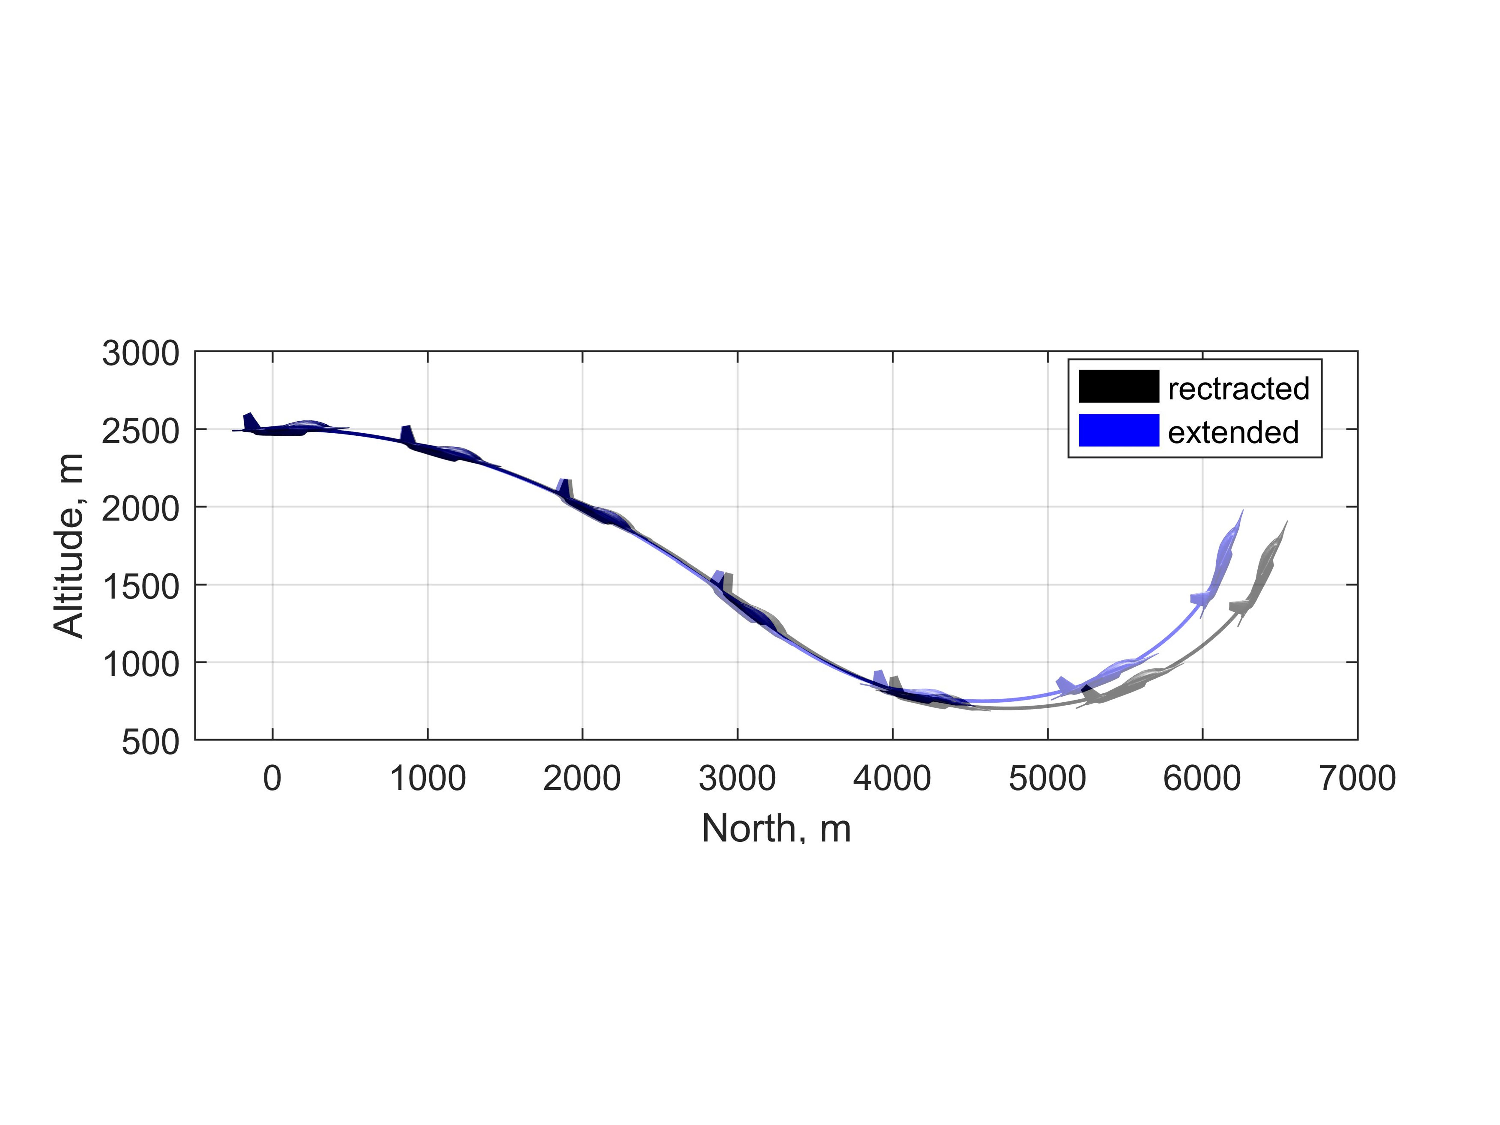
\includegraphics[width=0.6\textwidth]{./resources/pdf/pushover_trj.pdf}
		\caption{Pushover maneuver trajectory.}
		\label{fig:pushover_trj}
		\centering
		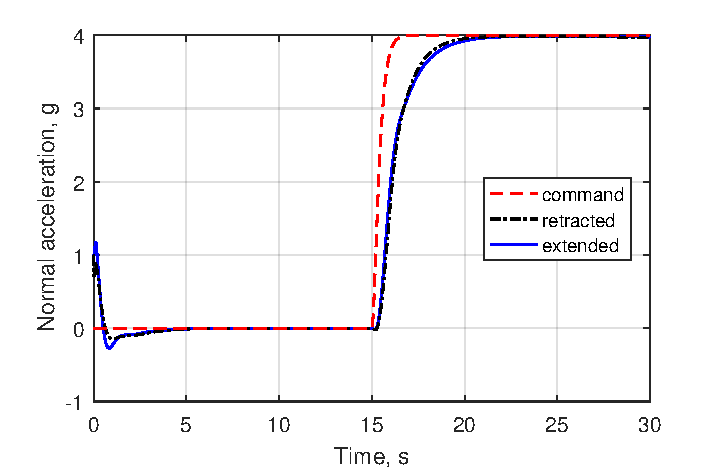
\includegraphics[width=0.6\textwidth]{./resources/pdf/pushover.pdf}
		\caption{Normal acceleration in pushover maneuver.}
		\label{fig:pushover}
	\end{figure}
	
	\section{Issues in Application to Morphing Aircraft}
	
	앞서 기술한 바와 같이 비선형 동적 모델역변환 제어기법은 일반적으로 비선형 시불변 시스템에 적용되어지는 제어방법론이다. 그렇기 때문에 특정 형상의 항공기에 대해 설계된 비선형 동적 모델역변환 제어기는 대규모로 형상이 변화한 항공기에 대해서는 안정성과 성능을 전혀 보장 할 수 없다. 그리고 모핑 항공기와 같은 비선형 시변 시스템에 비선형 동적 모델역변환 제어기법을 적용하기에는 제어기 설계의 복잡도가 매우 높아지는 어려움이 발생한다. 이러한 어려움은 성능 출력을 반복적으로 미분하는 과정 즉, Eq.~ \eqref{Eq:output_dere}을 계산하는 과정에서 다양한 시변 항들이 추가적으로 고려되어져야 한다는 사실로 부터 기인한다. 이 같은 어려움을 완화하기 위해서는 형상 변화에 따라 변하는 물리량들 중에서 변화량이 큰 물리량과 변화량이 작은 물리량을 구분하고 변화가 작은 물리량들은 적절한 상수 값으로 근사하여 시변항들을 최소화하고 이를 통해 설계 복잡도를 낮추는 것이 중요하다. 그러나 시변항들을 적절한 상수 값으로 근사화하더라도 상태공간 전체에서 만족스러운 제어 성능을 보장하는 비선형 동적 모델역변환 제어기를 설계하는 것은 여전히 복잡한 문제일 수 있다. 이를 해결하기위해서는 다양한 형태의 근사화된 비선형 동적 모델역변환 제어기법이 고려될 수 있을 것이다.
	
	\chapter{Conclusion}
	
	본 문서에서는 모핑 항공기의 수학적 모델을 도출하고 이를 기반으로 선형 및 비선형 제어기법을 적용하는 과정에 대해 기술하였다.
	또한 수치 시뮬레이션을 통해 기술된 기법이 모핑 항공기의 적절한 비행제어 성능을 만족시킴을 보였다.
	이러한 기법들은 가변스팬 모핑 항공기뿐만 아니라 유한한 형상변형 자유도를 가진 어떠한 형태의 모핑 항공기에도 적용될 수 있다.
	
	\printbibliography
	
	\appendix
	
	\chapter{MATLAB Code - LQR}
	
	\begin{table}[h]
		\centering
		\begin{tabular}{ll}
			\toprule
			\textbf{Variable} & \textbf{Description} \\
			\midrule
			\verb+alpha+ & Angle of attack (rad)\\
			\verb+q+ & Pitch rate (rad/s) \\
			\verb+V_T+ & True airspeed (m/s) \\
			\verb+theta+ & Pitch angle (rad) \\
			\verb+beta+ & Sideslip angle (rad) \\
			\verb+phi+ & Roll angle (rad) \\
			\verb+p+ & Roll rate (rad/s) \\
			\verb+r+ & Yaw rate (rad/s) \\
			\verb+A_lon+ & 4$\times$4 longitudinal system matrix \\
			\verb+B_lon+ & 4$\times$2 longitudinal input matrix \\
			\verb+Q_lon+ & 4$\times$4 longitudinal state weighting matrix \\
			\verb+R_lon+ & 2$\times$2 longitudinal input weighting matrix \\
			\verb+A_lat+ & 4$\times$4 lateral system matrix \\
			\verb+B_lat+ & 4$\times$2 lateral input matrix \\
			\verb+Q_lat+ & 4$\times$4 lateral state weighting matrix \\
			\verb+R_lat+ & 2$\times$2 lateral input weighting matrix \\
			\bottomrule
		\end{tabular}
		\caption{List of the variables in LQR.}
		\label{tab:lqr_variables}
	\end{table}
	
	\pagebreak
	
	\FrameTBStyle{matlab}
	\begin{lstlisting}[style=matlabFrameTB, gobble=4]
		% States
		x_lon = [alpha q V_T theta];
		x_lat = [beta phi p r];
		
		% Kalman gains
		[K_lon,~,~] = LQR(A_lon(eta),B_lon(eta),Q_lon,R_lon,~);
		[K_lat,~,~] = LQR(A_lat(eta),B_lat(eta),Q_lat,R_lat,~);
		
		% Optimal inputs
		u_lon = -K_lon*x_lon;
		u_lat = -K_lat*x_lat;
		
		% Control surface deflection commands
		dele_c = u_lon(1);
		delt_c = u_lon(2);
		dela_c = u_lat(1);
		delr_c = u_lat(2);
	\end{lstlisting}
	
	\chapter{MATLAB Code - NDI}
	
	\begin{table}[h]
		\centering
		\begin{tabular}{ll}
			\toprule
			\textbf{Variable} & \textbf{Description} \\
			\midrule
			\verb+phi_ref+ & Reference roll angle (rad) \\
			\verb+theta_ref+ & Reference pitch angle (rad) \\
			\verb+beta_ref+ & Reference sideslip angle (rad) \\
			\verb+phi+ & Roll angle (rad) \\
			\verb+theta+ & Pitch angle (rad) \\
			\verb+beta+ & Sideslip angle (rad) \\
			\verb+angle_err_int+ & Angle error integration (rad$\cdot$s) \\
			\verb+angle_err_dot+ & Angle error derivative (rad/s) \\
			\verb+K_P_i,K_I_i,K_D_i+ & 3$\times$3 PID gain matrices (i=1,2) \\
			\verb+X,Y,Z+ & Body-axis forces (N) \\
			\verb+m+ & Mass (kg) \\
			\verb+g+ & Gravitational acceleration (m/s$^2$) \\
			\verb+u,v,w+ & Body-axis velocity components (m/s) \\
			\verb+V_T+ & True airspeed (m/s) \\
			\verb+I+ & 3$\times$3 inertia matrix function (kg$\cdot$m$^2$) \\
			\verb+eta+ & Morphing parameter \\
			\verb+S+ & Planform area (m$^2$) \\
			\verb+b+ & Span (m) \\
			\verb+cbar+ & Mean aerodynamic chord (m) \\
			\verb+Cl,Cm,Cn+ & Moment coefficient functions \\
			\bottomrule
		\end{tabular}
		\caption{List of the variables in NDI.}
		\label{tab:ndi_variables}
	\end{table}
	
	\pagebreak
	
	\begin{lstlisting}[style=matlabFrameTB, gobble=4]
		% Reference angle derivatives
		angle_ref = [phi_ref;theta_ref;beta_ref];
		angle = [phi;theta;beta];
		angle_err = angle_ref-angle;
		angle_err_dot = angle_ref_dot-angle_dot;
		angle_ref_dot = K_P_1*angle_err+K_I_1*angle_err_int+K_D_1*angle_err_dot;
		
		% Body-axis accelerations
		ax = X/m - g*sin(theta);
		ay = Y/m + g*sin(phi)*cos(theta);
		az = Z/m + g*cos(phi)*cos(theta);
		
		% Intermediate matrix
		H = [1 sin(phi)*tan(theta) cos(phi)*tan(theta);
		0 cos(phi) -sin(phi);
		w/(sqrt(u^2+w^2)) 0 -u/(sqrt(u^2+w^2))];
		
		% Reference angular velocity       
		pqr_ref = inv(H)*(angle_ref_dot-...
		[0;0;(1/(sqrt(u^2+w^2)))*((-u*v/(V_T^2)*ax+...
		(1-(v^2)/(V_T^2))*ay-(v*w/(V_T^2))*az))];
		
		% Reference angular velocity derivatives
		pqr_ref_dot = K_P_2*pqr_err+K_I_2*pqr_err_int+K_D_2*pqr_err_dot;
		
		% Required moments
		lmn_req = I(eta)*pqr_ref + cross(pqr,I(eta)*pqr);
		
		% Required moment coefficients
		Cl_req = lmn_req(1)/(0.5*rho*(V_T^2)*S*b);
		Cm_req = lmn_req(2)/(0.5*rho*(V_T^2)*S*cbar);
		Cn_req = lmn_req(3)/(0.5*rho*(V_T^2)*S*b);
		
		% Required control surface deflections
		del_req = inv([Cl_dela Cl_dele Cl_delr;Cm_dela Cm_dele Cm_delr;
		Cn_dela Cn_dele Cn_delr])*...
		([Cl_req;Cm_req;Cn_req]-[Cl(eta);Cm(eta);Cn(eta)]);
		
		% Control surface deflection commands
		dele_c = del_req(1);
		dela_c = del_req(2);
		delr_c = del_req(3);
	\end{lstlisting}

\end{document}
